\documentclass{report}
\usepackage[utf8]{inputenc}
\usepackage[T2A]{fontenc}
\usepackage[russian]{babel}
\usepackage{graphicx}
\usepackage{amsmath}
\usepackage{amsfonts}
\usepackage{amssymb}
\usepackage{bm}

\usepackage{mathtools}
\newcommand\iid{\stackrel{\mathclap{\normalfont\mbox{iid}}}{\sim}}

\setcounter{chapter}{1}


\title{Введение в Бутстреп}
% \author{st013309}
\date{2021}

\begin{document}

\maketitle
\begin{center}
	\textbf{Глава 8}\\
\end{center}
\textbf{Более сложные структуры данных}\\
\textbf{8.1 Введение}\\
Алгоритм бутстрепа на рисунке 6.1 основан на простейшей возможной вероятностной модели для случайных данных: одновыборочная модель, в которой одно неизвестное вероятностное распределение $F$ порождает данные $\textbf{x}$ путем случайной выборки.
$$F \to \textbf{x} = (x_1, x_2, \cdots , x_n). \eqno(8.1)$$
Отдельные единицы данных $x_i$ в (8.1) сами по себе могут быть довольно сложными, возможно, в виде чисел, векторов, карт, изображений или чего-то еще, но сам вероятностный механизм прост. Многие задачи анализа данных связаны с более сложными структурами данных. Эти структуры имеют такие названия, как временные ряды, дисперсионный анализ, регрессионные модели, многовыборочные задачи, цензурированные данные, стратифицированная выборка и т.д. Алгоритм бутстрепа можно адаптировать к общим структурам данных, как это обсуждается здесь и в главе 9.\\
\textbf{8.2 Одновыборочные задачи}\\
На рис. 8.1 представлена схематическая диаграмма метода бутстрепа применительно к одновыборочным задачам. Слева --- реальный мир, где неизвестное распределение $F$ породило наблюдаемые данные $\textbf{x} = (x_1, x_2, \cdots, x_n)$ путем генерации случайной выборки. Мы вычислили интересующую статистику из $\textbf{x}, \hat{\theta} = s(\textbf{x})$, и хотим узнать что-нибудь о статистическом поведении $\hat{\theta}$, возможно, о его стандартной ошибке $\text{se}_F (\hat{\theta})$.

В правой части рисунка находится мир бутстрепа, если использовать запоминающуюся терминологию Дэвида Фридмана. В мире бутстрепа эмпирическое распределение $\hat{F}$ порождает бутстреп выборки $\textbf{x}:* = (x_1^*, x_2^*, \cdots, \\ x_n^*)$ путем генерации случайной выборки, на основе которой мы вычисляем бутстреп репликации интересующей статистики, $\hat{\theta}^* = s(\textbf{x}^*)$. Большим преимуществом мира бутстрепа является то, что мы можем вычислить столько репликаций $\hat{\theta}^*$, сколько захотим, или, по крайней мере, столько, сколько мы можем себе позволить. Это позволяет нам делать вероятностные вычисления напрямую, например, используя наблюдаемую изменчивость $\hat{\theta}^*$ для оценки ненаблюдаемой величины $\text{se}_F(\hat{\theta})$.

Двойная стрелка на рис. 8.1 указывает на вычисление $\hat{F}$ из $F$. По идее, это решающий шаг в процессе бутстрепа, даже несмотря на то, что он прост в вычислительном отношении. Любая другая часть картины бутстрепа определяется аналогично: $F$ порождает $\textbf{x}$ путем генерации случайной выборки, поэтому $\hat{F}$ порождает $\textbf{x}^*$ путем генерации случайной выборки; $\hat{\theta}$ получается из $\textbf{x}$ через функцию $s(\textbf{x})$, поэтому $\hat{\theta}^*$ получается из $\textbf{x}^*$ таким же образом. Расчеты бутстрепа для более сложных вероятностных механизмов оказываются простыми, если мы знаем, как реализовать процесс, обозначенный двойной стрелкой --- оценку всего вероятностного механизма на основе данных. К счастью, это легко сделать для всех распространенных структур данных.

\newpage

\noindent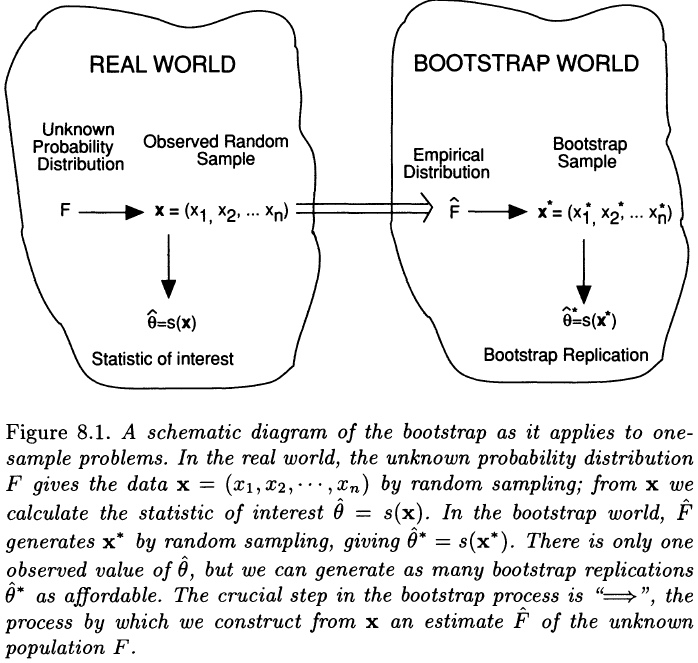
\includegraphics[width=12cm]{fig81}

Чтобы облегчить изучение более сложных структур данных, мы будем использовать обозначение
$$P \to \textbf{x} \eqno(8.2)$$
чтобы указать, что неизвестная \textit{вероятностная модель} $P$ породила наблюдаемый набор данных $\textbf{x}$.\\
\textbf{8.3 Двувыборочная задача}\\
Чтобы понять обозначения (8.2), рассмотрим данные о мышах в таблице 2.1. Вероятностную модель $P$ можно представить как пару распределений вероятностей $F$ и $G$, первое для экспериментальной группы и второе для контрольной группы,

$$P = (F, G). \eqno(8.3)$$

Пусть $\textbf{z} = (z_1, z_2, \cdots, z_m)$ обозначает экспериментальные наблюдения, а $\textbf{y} = (y_1, y_2, \cdots, y_n)$ обозначает контрольные наблюдения с $n = 7$ и $m = 9$. Тогда наблюдаемые данные включают $\textbf{z}$ и $\textbf{y}$,
$$\textbf{x} = (\textbf{z}, \textbf{y}). \eqno(8.4)$$
Мы можем думать об $\textbf{x}$ как о $16$-мерном векторе, если мы помним, что первые семь координат исходят из $F$, а последние девять --- из $G$. Отображение $P \to x$ описывается следующим образом:
$$F \to \textbf{z} \text{ независимо от } G \to \textbf{y}. \eqno(8.5)$$
Другими словами, $\textbf{z}$ --- это случайная выборка размера $7$ из $F$, $\textbf{y}$ --- случайная выборка размера $9$ из $G$, причем $\textbf{z}$ и $\textbf{y}$ взаимно независимы друг от друга. Такая постановка называется \textit{двухвыборочной задачей}. 

В этом случае легко оценить вероятностный механизм $P$. Пусть $\hat{F}$ и $\hat{G}$ --- эмпирические распределения, основанные на $\textbf{z}$ и $\textbf{y}$ соответственно. Тогда естественная оценка $P = (F, G)$ такова:

$$\hat{P} = (\hat{F}, \hat{G}). \eqno(8.6)$$

После получения $\hat{P}$ определение бутстреп выборки $\textbf{x}^*$ очевидно: стрелка в
$$\hat{P} \to \textbf{x}^* \eqno(8.7)$$
должна означать то же самое, что и стрелка в $P \to \textbf{x}$, (8.2). В двухвыборочной задаче (8.5) мы имеем $\textbf{x}^* = (\textbf{z}^*, \textbf{y}^*)$, где
$$\hat{F} \to \textbf{z}^* \text{ независимо от } \hat{G} \to \textbf{y}^*. \eqno(8.8)$$
Размеры выборки для $\textbf{z}^*$ и $\textbf{y}^*$ такие же, как для $\textbf{z}$ и $\textbf{y}$ соответственно.

На Pисунке 8.2 показана гистограмма $B = 1400$ бутстреп репликаций статистики $\hat \theta$
 	
\begin{tabular}{ l l l }
	$\hat{\theta}$ & = & $\hat{\mu}_z - \hat{\mu}_y = \bar{z} - \bar{y}$ \\
				   & = & $86.86 - 56.22 = 30.63,$ \\
\end{tabular}

$$\eqno(8.9)$$
где $\hat \theta$ --- разность в средних значениях экспериментальной и контрольной групп в данных о мышах. Эта статистика оценивает параметр
$$\theta = \mu_z - \mu_y = \text{E}_f(z) - \text{E}_G(y). \eqno(8.10)$$
Если $\theta$ действительно намного больше $0$, как, по-видимому, указывает (8.9), то экспериментальная группа показывает гораздо лучший результат по сравнению с контрольной группой. Однако бутстреп оценка стандартной ошибки для $\hat{\theta} = 30.63$ это 
$$\hat{\text{se}}_{1400} = \{ \sum_{b=1}^{1400} [ \hat{\theta}^*(b) - \hat{\theta}^*(\cdot) ]^2 / 1399 \}^{1/2} = 26.85, \eqno(8.11)$$
поэтому $\hat{\theta}$ всего лишь на $1.14$ стандартной ошибки больше нуля, $1.14 = 30.63 / 26.85$. Обычно такой результат не считается убедительным доказательством того, что истинное значение $\theta$ больше $0$.

Бутстреп репликации $\hat{\theta}^*$ были получены при помощи генератора случайных чисел для соблюдения независимости (8.8). Каждая бутстреп выборка $\textbf{x}^*$ была вычислена следующим образом
$$\textbf{x}^* = (\textbf{z}^*, \textbf{y}^*) = (z_{i_1}, z_{i_2}, \cdots, z_{i_7}, y_{j_1}, y_{j_2}, \cdots, y_{j_9}), \eqno(8.12)$$
где $(i_1, i_2, \cdots, i_7)$ была случайной выборкой размера $7$ из целых чисел $1, 2, \cdots, 7$, а $(j_1, j_2, \cdots, j_g)$ была независимо выбранной случайной выборкой размера $9$ из целых чисел $1, 2, \cdots, 9$. Например, первая бутстреп выборка была $(i_1, i_2, \cdots, i_7) = (7,3,1,2,7,6,3)$ и $(j_1, j_2, \cdots, j_9) = (7,8,2,9,6,7,8,4,2)$.

Стандартная ошибка $\theta$ может быть записана как $\text{se}_P(\hat{\theta})$, чтобы обозначить ее зависимость от неизвестного вероятностного механизма $P = (F, G)$. Бутстреп оценка $\text{se}_P(\hat{\theta})$ --- это оценка методом подстановки
$$\text{se}_{\hat{P}}(\hat{\theta}^*) = \{ \text{var}_{\hat{P}}(\bar{z}^* - \bar{y}^*) \}^{1/2}. \eqno(8.13)$$
Как и в главе 6, мы аппроксимируем идеальную бутстреп оценку $\text{se}_{\hat{P}}(\hat{\theta}^*)$ при помощи $\hat{\text{se}}_B$ из уравнения (6.6), в данном случае при $B = 1400$. Тот факт, что $\hat{\theta}^*$ вычисляется из двух выборок, $\textbf{z}^*$ и $\textbf{y}^*$ не влияет на определение (6.6), а именно $\hat{\text{se}}_B = \{ \sum_{b=1}^{B} [\hat{\theta}^*(b) - \hat{\theta}^*(\cdot)]^2/(B-1) \}^{1/2}$.\\
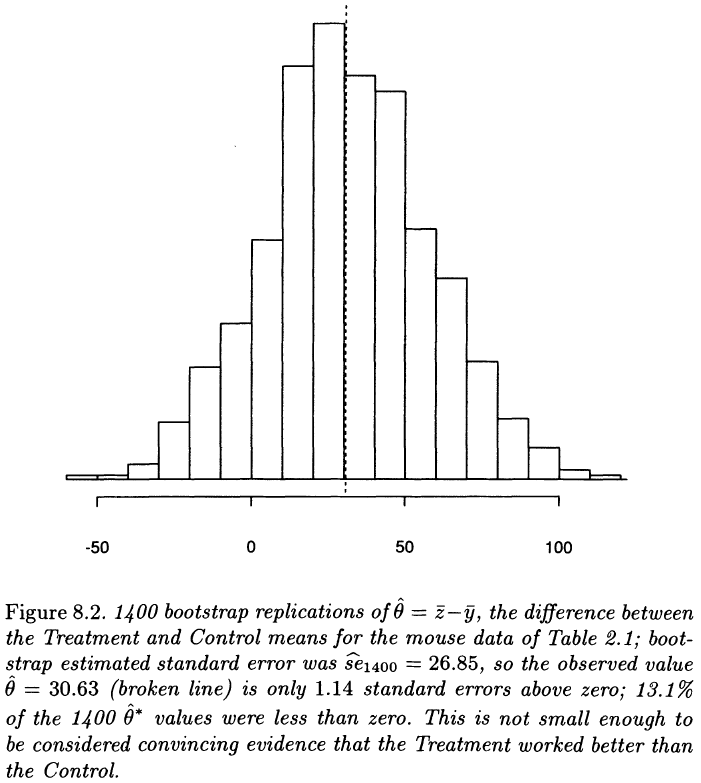
\includegraphics[width=12cm]{fig82}\\
\textbf{8.4 Более общие структуры данных}\\
Рисунок 8.3 --- это версия рисунка 8.1, который применяется к общим структурам данных $P \to \textbf{x}$. Между этими двумя рисунками нет особой концептуальной разницы, за исключением уровня обобщения. В реальном мире неизвестный вероятностный механизм $P$ порождает наблюдаемый набор данных $\textbf{x}$ в соответствии с правилом построения, указанным стрелкой «$\to$». В конкретных приложениях нам нужно более тщательно определять стрелку, наподобие того как в (8.5) для двухвыборочной задачи. Набор данных $\textbf{x}$ больше не может быть одним вектором. Он имеет форму, зависящую от структуры данных, например $\textbf{x} = (\textbf{z}, \textbf{y})$ в двухвыборочной задаче. Наблюдая за $\textbf{x}$, мы вычисляем интересующую статистику $\hat{\theta}$ из $\textbf{x}$ в соответствии с функцией $s(\cdot)$.\\
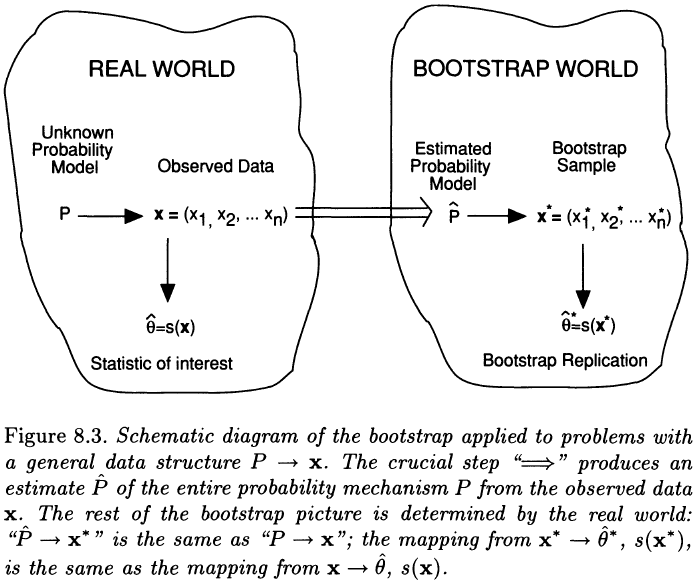
\includegraphics[width=12cm]{fig83}

Бутстреп часть на рис. 8.3 описывается аналогичными понятиями и в реальном мире: стрелка в $\hat{P} \to \textbf{x}^*$ означает то же самое, что и стрелка в $P \to \textbf{x}$. И функция, отображающая $\textbf{x}^*$ в $\hat{\theta}^*$, является той же функцией $s(\cdot)$, что и отображающая $\textbf{x}$ в $\hat{\theta}$. 

При фактическом проведении бутстреп анализа на основе рисунка 8.3 возникают две практические задачи:

(1) Нам нужно оценить весь вероятностный механизм $P$ по наблюдаемым данным $\textbf{x}$. Это шаг, обозначенный двойной стрелкой $\textbf{x} \Rightarrow \hat{P}$. Это удивительно легко сделать для большинства знакомых структур данных. Универсального рецепта нет, но в каждом отдельном случае доступны вполне обычные конкретные решения, например, $\hat{P} = (\hat{F}, \hat{G})$ для двухвыборочной задачи. Дополнительные примеры приведены в этой и следующей главах.

(2) Нам нужно смоделировать бутстреп данные из $\hat{P}$ в соответствии с подходящей структурой данных. Это шаг $\hat{P} \to \textbf{x}^*$ изображен на рисунке 8.3. Этот шаг концептуально прост, будучи такм же, как $P \to \textbf{x}$, но может потребовать некоторой осторожности при программировании, если необходима вычислительная эффективность. (Мы увидим пример в анализе лютенизирующего гормона ниже.) Обычно генерация бутстреп данных $\hat{P} \to \textbf{x}^*$ требует меньше времени, часто гораздо меньше времени, чем вычисление $\hat{\theta}^* = s(\textbf{x}^*)$.\\
\begin{center}
	Таблица 8.1. \textit{Данные лютеинизирующего гормона.}
\end{center}
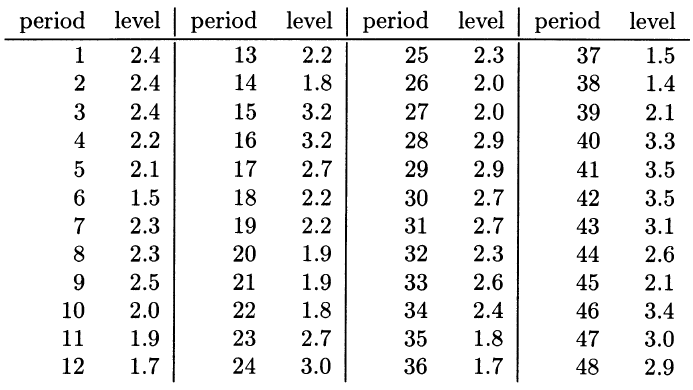
\includegraphics[width=12cm]{tab81}\\
\textbf{8.5 Пример: лютеинизирующий гормон}\\
На рис. 8.4 показан набор уровней $y_t$ лютенизирующего гормона для каждого из $48$ отрезков времени, взятых из Diggle (1990); набор данных приведен в таблице 8.1. Это уровни гормонов, измеренные у здоровой женщины с $10$-минутными интервалами в течение $8$ часов. Лютенизирующий гормон является одним из гормонов, регулирующих менструальный цикл, и поэтому важно понимать его суточные колебания. 

Понятно, что уровни гормонов не являются случайной выборкой из какого-либо распределения. На рисунке 8.4 слишком много данных. Эти данные являются примером \textit{временного ряда}: структуры данных, для которой близкие значения временного параметра $t$ указывают тесно связанные значения измеренной величины $y_t$. Многие интересные вероятностные модели использовались для анализа временных рядов. Мы начнем с простейшей модели --- \textit{схемы авторегрессии первого порядка}.

Пусть $\mu$ --- математическое ожидание $y_t$, которое предполагается одинаковым для всех моментов времени $t$, и определим \textit{центрированные} измерения
$$z_t = y_t - \mu. \eqno(8.14)$$
Все $z_t$ имеют математическое ожидание $0$. Схема авторегрессии первого порядка --- это одна из таких схем, в которой каждый $z_t$ является линейной комбинацией предыдущего значения $z_{t-1}$ и независимого шума $\varepsilon_t$, 
$$z_t = \beta z_{t-1} + \varepsilon_t \text{ для } t = U, U + 1, U + 2, \cdots, V. \eqno(8.15)$$
Здесь $\beta$ --- неизвестный параметр, действительное число от $-1$ до $1$. 

Предполагается, что шум $\varepsilon_t$ в (8.15) является случайной выборкой из неизвестного распределения $F$ с математическим ожиданием $0$,
$$F \to (\varepsilon_U, \varepsilon_{U+1}, \varepsilon_{U+2}, \cdots, \varepsilon_V) \quad [\text{E}_F(\varepsilon) = 0]. \eqno(8.16)$$
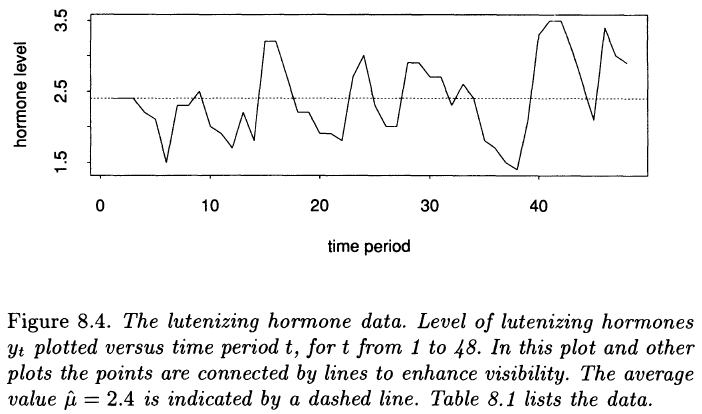
\includegraphics[width=12cm]{fig84}\\
Точки $U$ и $V$ --- это начало и конец анализируемого периода времени. Здесь у нас есть
$$U = 2 \text{ и } V = 48. \eqno(8.17)$$
Обратите внимание, что первое уравнение в (8.15) имеет вид 
$$z_U = \beta z_{U-1} + \varepsilon_U, \eqno(8.18)$$
поэтому нам нужно число $z_{U-1}$, чтобы запустить процесс авторегрессии. В нашем случае $z_{U-1} = z_1$. 

Пусть мы считаем, что модель (8.15), (8.16), авторегрессионный процесс первого порядка, применима к данным лютенизирующего гормона. Как мы можем оценить значение $\beta$ по данным? Один из ответов основан на методе наименьших квадратов. Прежде всего, мы оцениваем математическое ожидание $\mu$ в (8.14) по наблюдаемому среднему значению $\bar{y}$ (это $2.4$ для данных лютенизирующего гормона) и устанавливаем 
$$z_t = y_t - \bar{y} \eqno(8.19)$$
для всех значений $t$. В дальнейшем мы проигнорируем разницу между определениями (8.14) и (8.19), см. задачу 8.4. 

Предположим, что $b$ --- это любое предположение об истинном значении $\beta$ в (8.15). Определим остаточную квадратичную ошибку для этого предположения как
$$\text{RSE}(b) = \sum_{t=U}^{V} (z_t - b_{z_{t-1}})^2. \eqno(8.20)$$
Используя (8.15) и тот факт, что $\text{E}_F(\varepsilon) = 0$, легко показать, что $\text{RSE}(b)$ имеет математическое ожидание $\text{E}(\text{RSE}(b)) = (b-\beta)^2 \text{E}(\sum_{t=U}^{V} z_{t-1}^2) + (V-U+1) \text{var}_F(\varepsilon)$. Оно минимизируется, когда $b$ равно истинному значению $\beta$. Мы убедились, что $\text{RSE}(b)$ должен достичь своего минимума где-то рядом с истинным значением $\beta$. 

Учитывая данные временного ряда, мы можем рассчитать $\text{RSE}(b)$ как функцию $b$, и выбрать минимизирующее значение, которое будет нашей оценкой $\beta$,
$$\text{RSE}(\hat{\beta}) = \min_b \text{RSE}(b). \eqno(8.21)$$
Данные по лютенизирующему гормону имеют следующую оценку наименьших квадратов

$$\hat{\beta} = 0.586. \eqno(8.22)$$

Насколько точна оценка $\hat{\beta}$? Чтобы ответить на этот вопрос, мы можем использовать общую бутстреп процедуру, показанную на рис. 8.3. Вероятностный механизм $P$, описанный в (8.15), (8.16), имеет два неизвестных элемента, $\beta$ и $F$, скажем, $P = (\beta, F)$. (Здесь мы рассматриваем $\mu$ в (8.14) как известную и равную $\bar{y}$.) Данные $\textbf{x}$ состоят из наблюдений $y_t$ и соответствующих им периодов времени $t$. Мы знаем, что правило построения $P \to \textbf{x}$ описывается формулами (8.15)--(8.16). Интересующая статистика $\hat{\theta}$ равна $\hat{\beta}$, поэтому отображения $s(\cdot)$ неявно задаются (8.21).

Остается один шаг, прежде чем мы сможем выполнить алгоритм бутстрепа: шаг двойной стрелки $\textbf{x} \Rightarrow \hat{P}$, в котором $P = (\beta, F)$ оценивается по данным. Теперь $\beta$ уже была оценена с помощью $\hat{\beta}$, (8.21), поэтому нам нужно только оценить \underline{распределение остатков} $F$. Если бы мы знали $\beta$, то мы могли бы вычислить $\varepsilon_t = z_t - \beta z_{t-1}$ для каждого $t$ и оценить $F$ по эмпирическому распределению значений $\varepsilon_t$. Мы не знаем $\beta$, но мы можем использовать оценочное значение $\hat{\beta}$, чтобы вычислить \underline{остатки}
$$\hat{\varepsilon}_t = z_t - \hat{\beta} z_{t-1} \text{ для } t = U, U + 1, U + 2, \cdots, V. \eqno(8.23)$$
Пусть $T = V - U + 1$, количество слагаемых в (8.23); $T = 47$ для выбора (8.17). Очевидная оценка $F$ --- это $\hat{F}$, эмпирическое \underline{распределение остатков}

$$\hat{F}: \text{ вероятность } 1/T \text{ для } \hat{\varepsilon}_t \text{ при } t = U, U + 1, \cdots, V. \eqno(8.24)$$

На рис. 8.5 показана гистограмма \underline{остатков} $\hat{\varepsilon}_t = z_t - \hat{\beta} z_{t-1}$ с $T = 47$ для схемы авторегрессии первого порядка, примененной к лютеинизирующим данным в промежутке 2--48 лет.\\
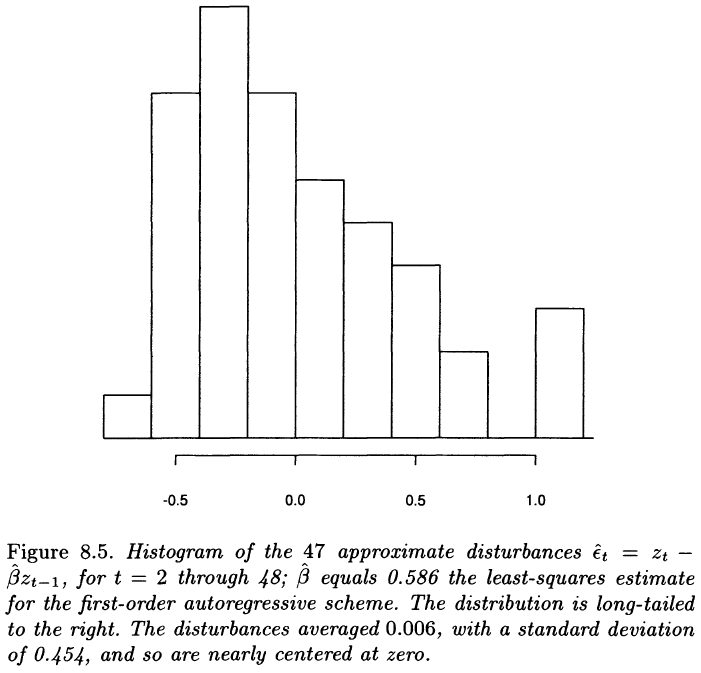
\includegraphics[width=12cm]{fig85}

Мы видим, что распределение $\hat{F}$ не является нормальным и имеет длинный хвост справа. Распределение имеет среднее значение $0.006$ и стандартное отклонение $0.454$. Не случайно, что среднее значение $\hat{F}$ близко к $0$; см. задачу 8.5. Если бы это было не так, мы могли бы соблюдать определение $\text{E}_F(\varepsilon) = 0$ в (8.16) путём центрирования $\hat{F}$; то есть изменением каждой вероятностной точки в (8.23) от $\hat{\varepsilon}_t$ до $\hat{\varepsilon}_t - \bar{\varepsilon}$, где $\bar{\varepsilon} = \sum_{U}^{V} \hat{\varepsilon}_t/T$.

Теперь мы готовы провести бутстреп анализ точности оценки $\hat{\beta} = 0.586$. Набор бутстреп данных $\hat{P} \to \textbf{x}^*$ генерируется в соответствии с определениями (8.15)--(8.16), за исключением $\hat{P} = (\hat{\beta}, \hat{F})$, заменённого на $P = (\beta, F)$. Начнем с начального значение $z_1 = y_1 - \bar{y}$, которое считается фиксированной константой (как размер выборки $n$ в одновыборочной задаче). Бутстреп временной ряд $z_t^*$ вычисляется рекурсивно,

\begin{tabular}{ l l l }
	$z_2^*$ & = & $\hat{\beta} z_1 + \varepsilon_2^*$ \\
	$z_3^*$ & = & $\hat{\beta} z_2^* + \varepsilon_3^*$ \\
	$z_4^*$ & = & $\hat{\beta} z_3^* + \varepsilon_4^*$\\
	$\vdots$ & & $\vdots$\\
	$z_{48}^*$ & = & $\hat{\beta} z_{47}^* + \varepsilon_{48}^*.$\\
\end{tabular}

$$\eqno(8.25)$$
Бутстреп остатки $\varepsilon_t^*$ представляют собой случайную выборку из $\hat{F}$,
$$\hat{F} \to (\varepsilon_2^*, \varepsilon_2^*, \cdots, \varepsilon_{48}^*). \eqno(8.26)$$
Другими словами, каждый $\varepsilon_t^*$ равняется любому из $T$ \underline{остатков} (8.23) с вероятностью $1/T$.

Процесс бутстрепа (8.25)--(8.26) был запущен $B=200$ раз, что дало $200$ бутстреп временных рядов. Каждый из них дал бутстреп репликацию $\hat{\beta}^*$ для оценки $\hat{\beta}$ методом наименьших квадратов, (8.21). На рисунке 8.6 показана гистограмма из $200$ значений $\hat{\beta}^*$. Оценка бутстреп стандартной ошибки для $\hat{\beta}$ составляет $\hat{\text{se}}_{200} = 0.116$. Гистограмма имеет довольно нормальную форму.
				
В схеме авторегрессии первого порядка каждый $z_t$ зависит от своих предшественников только через значение $z_{t-1}$ (Этот вид зависимости известен как \textit{марковский процесс первого порядка}.) Схема авторегрессии второго порядка расширяет зависимость обратно до $z_{t-2}$,
$$z_t = \beta_1 z_{t-1} + \beta_2 z_{t-2} + \varepsilon_t$$
$$\text{для } t = U, U + 1, U + 2, \cdots, V. \eqno(8.27)$$
Здесь $\bm \beta = (\beta_1, \beta_2)^\text{T}$ --- двумерный вектор неизвестных параметров. $\varepsilon_t$ --- независимые \underline{остатки}, как в (8.16). Согласно (8.18) исходные уравнения следующие 
$$z_U = \beta_1 z_{U-1} + \beta_2 z_{U-2} + \varepsilon_U$$
$$z_{U+1} = \beta_1 z_U + \beta_2 z_{U-1} + \varepsilon_{U+1}, \eqno(8.28)$$
поэтому нам нужны числа $z_{U-2}$ и $z_{U-1}$ для начала. Теперь $U = 3$, $V = 48$ и $T = V - U + 1 = 46$.

Метод наименьших квадратов непосредственно приводит к оценке вектора $\bm{\beta}$. Пусть $\textbf{z}$ является $T$-мерным вектором $(z_U, z_{U+1}, \cdots, z_V)^\text{T}$, и пусть $\textbf{Z}$ --- матрица $T \times 2$ с первым столбцом $(z_{U-1}, z_U, \cdots, z_{V-1})^\text{T}$, вторым столбцом $(z_{U-2}, z_{U-1}, z_U,  \cdots, z_{V-2})^\text{T}$. Тогда оценка $\bm{\beta}$ методом наименьших квадратов следующая

$$\hat{\bm \beta} = (\textbf{Z}^\text{T} \textbf{Z})^{-1} \textbf{Z}^\text{T} \textbf{z}. \eqno(8.29)$$

Для данных о лютенизирующем гормоне схема авторегрессии второго порядка имела слуедующие оценки наименьших квадратов
$$\hat{\bm \beta} = (0.771, -0.222)^\text{T}. \eqno(8.30)$$
На рис. 8.7 показаны гистограммы с $B=200$ бутстреп репликациями из двух компонентов из $\hat{\bm \beta} = (\hat{\beta}_1, \hat{\beta}_2)^\text{T}$. Стандартные ошибки бутстрепа равны
$$\hat{\text{se}}_{200} (\hat \beta_1) = 0.147, \quad \hat{\text{se}}_{200} (\hat \beta_2) = 0.149. \eqno(8.31)$$\\
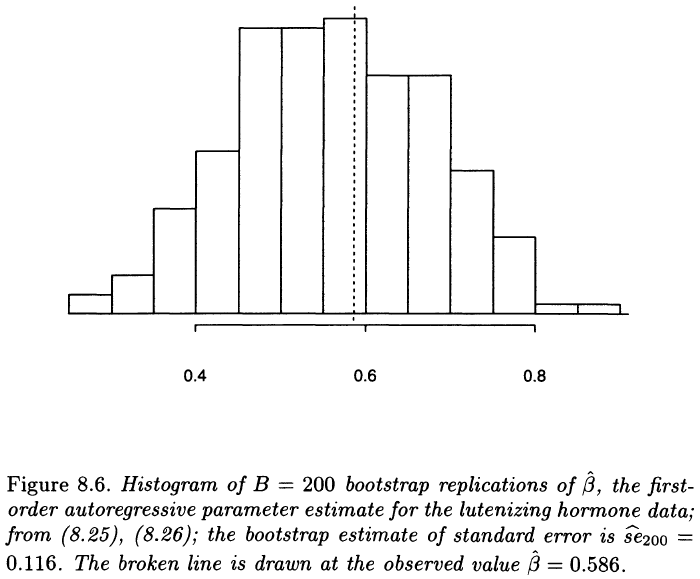
\includegraphics[width=12cm]{fig86}

Обе гистограммы имеют примерно нормальную форму. В задаче 8.7 читателю требуется описать шаги, ведущие к рисунку 8.7.
	
Схема авторегрессии второго порядка $\beta_2 = 0$ это схема авторегрессии первого порядка. При выполнении анализа точности для схемы второго порядка мы проверяем, не отклоняется ли $\hat \beta_2$ от $0$ менее чем на $2$ стандартных ошибки, что обычно интерпретируется как незначительное отличие $\hat \beta_2$ от $0$. Здесь $\hat \beta_2$ --- это примерно $1.5$ стандартные ошибки от $0$, и в этом случае у нас нет убедительных доказательств того, что схема авторегрессии первого порядка не дает разумного представления данных о лютеинизирующем гормоне.
		
Знаем ли мы наверняка, что схема первого порядка дает хорошее представление о ряде лютенизирующих гормонов? Мы не можем дать окончательный ответ на этот вопрос, не рассматривая еще более общие модели, такие как схемы авторегрессии более высоких порядков. Приблизительный ответ может быть получен путем сравнения бустреп временных рядов с фактическими рядами на рис. 8.4. На рисунке 8.8 на левых графиках показаны первые четыре бустраповых набора из первой схемы, правая часть графиков отображает четыре реализации, полученные путем выборки с заменой из исходного временного ряда. Исходные данные на рис. 8.4 очень похожи на реализации левых графиков и совсем не похожи на реализации правых графиков.\\
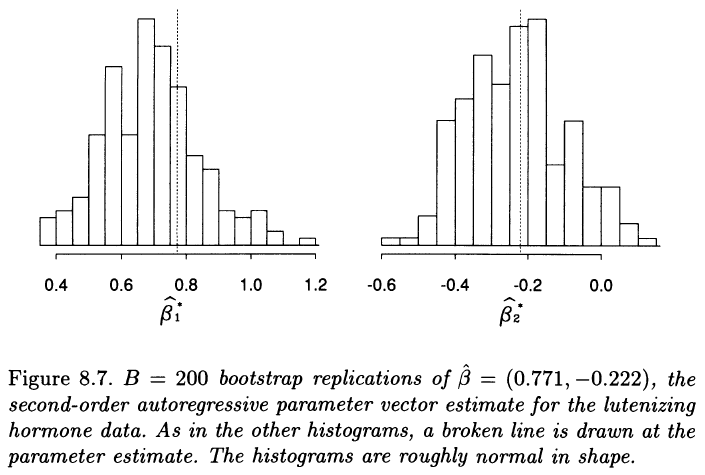
\includegraphics[width=12cm]{fig87}

Дальнейший анализ показывает, что модель AR(1) обеспечивает разумное соответствие этим данным. Однако нам потребуется более длительный временной ряд, чтобы эффективно различать разные модели этого гормона.

В общем, стоит помнить, что математические модели представляют собой удобные упрощенные представления сложных явлений реального мира и обычно не совсем корректны. Часто необходим некоторый компромисс между усложнением модели и научными потребностями исследования. Методы бустрепа особенно полезны, если существует потребность в сложных моделях, поскольку математическая сложность не является препятствием для анализа точности бустрепа.\\
\textbf{8.6 Бутстреп скользящих окон}\\
В этом последнем разделе мы кратко опишем другой метод бустрапирования временных рядов. Вместо подгонки модели и последующей выборки из остатков этот метод использует подход, более близкий к подходу, используемому для одновыборочных задач. Идея проиллюстрирована на рисунке 8.9. Исходный временной ряд представлен черными кружками. Чтобы сгенерировать бустреп реализацию временного ряда (белые кружки), мы выбираем длину окна («$3$» на диаграмме) и рассматриваем все возможные смежные окна этой длины. Мы составляем выборку с заменой из этих окон и объединяем их вместе, чтобы сформировать бутстреп временные ряды. Выбирается ровно столько окон, сколько необходимо для получения серии примерно такой же длины, что и исходная. Если длина окна равна $l$, то выберем $k$ окон так, чтобы $n \approx k \cdot l$.

Для иллюстрации мы выполним данные действия для данных о лютенизирующем гормоне. Интересующей статистикой была оценка $\hat \beta$ методом наименьших квадратов у AR(1). Мы выбрали длину окна $3$ и использовали\\ 
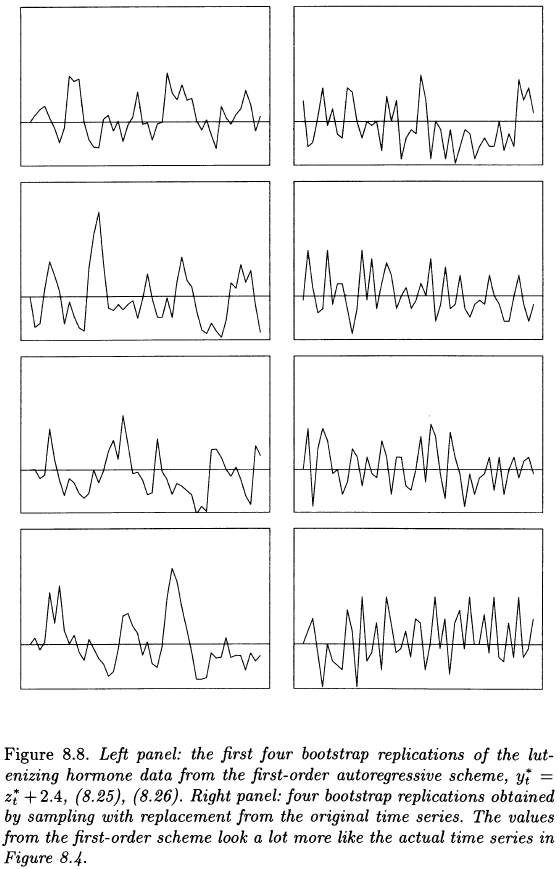
\includegraphics[width=12.5cm]{fig88}\\
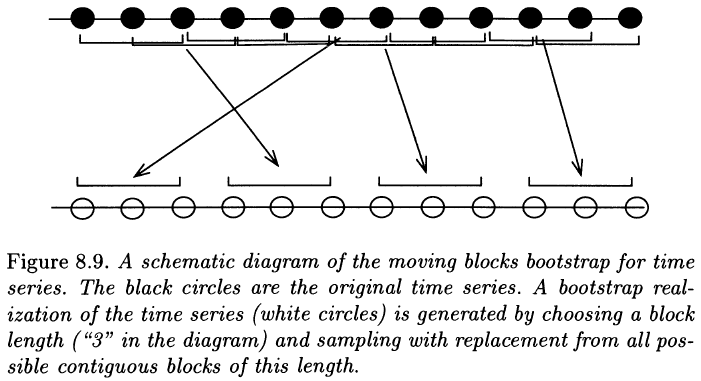
\includegraphics[width=12cm]{fig89}\\
бутстреп скользящих окон для генерации бустреп данных лютенизирующего гормона. Типичная реализация бустрепа показана на рисунке 8.10, и она очень похожа на исходный временной ряд. Затем мы подогнали модель AR(1) к этому бутстреп временному ряду и оценили коэффициент $\hat \beta^*$ у AR(1). Весь этот процесс был повторен $B=200$ раз. (Обратите внимание, что модель AR(1) используется здесь для оценки $\beta$, но не используется при генерации бустреп реализаций временного ряда.) В результате стандартная ошибка бустрепа составила $\widehat {\text{se}}_{200} (\hat \beta) = 0.120$. Это примерно то же самое, что и значение $0.116$, полученное из AR(1) выборок, сгенерированных в предыдущем разделе. Увеличение размера окна до $5$ привело к уменьшению этого значения до $0.103$.

Чем оправдан бутстреп скользящих окон? Как мы видели ранее, мы не можем просто создать повторную выборку из отдельных наблюдений, так как это разрушило бы корреляцию, на которой мы хотим сфокусировать внимание. (Использование размера окна, равного единице, соответствует выборке с возвращением, и дает $0.139$ для оценки стандартной ошибки.) С бутстрепом скользящих окон идея состоит в том, чтобы выбрать размер окна $l$ достаточно большим, чтобы наблюдения, отстоящие более чем на $l$ единиц времени, были почти независимыми. Выбирая окна длиной $l$, мы сохраняем корреляцию, присутствующую в наблюдениях, разделенных менее чем $l$ единиц.

Бутстреп скользящих окон имеет то преимущество, что он менее «зависим от модели», чем подход бутстреп остатков, использовавшийся ранее. Как мы видели, последний метод зависит от модели, которая соответствует исходному временному ряду (например, модель AR(1) или AR(2)). Однако выбор размера окна $l$ может быть весьма важным, и эффективные методы для этого еще не разработаны.

В задаче регрессии, обсуждаемой в следующей главе, мы сталкиваемся с различными методами бустрепа, аналогичными подходам для временных\\
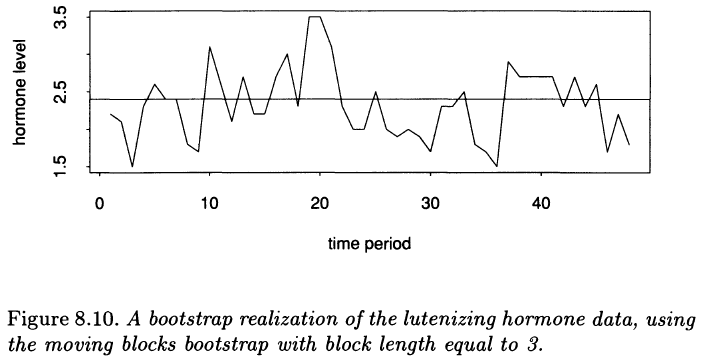
\includegraphics[width=12cm]{fig810}\\
рядов, которые мы обсуждали здесь.\\
\textbf{8.7 Библиографические примечания}\\
Анализ временных рядов описан во многих книгах, включая Box and Jenkins (1970), Chatfield (1980) и Diggle (1990). Применение бутстрепа к временным рядам обсуждается в Efron and Tibshirani (1986); Метод скользящих окон и связанные с ним техники можно найти у Carlstein (1986), Kiinsch (1989), Liu and Singh (1992) и Politis and Romano (1992).

\end{document}